\documentclass[convert={density=300,size=1080x800,outext=.png}]{standalone}

\usepackage{tikz}
\usetikzlibrary{decorations.pathreplacing}
\usetikzlibrary{arrows,positioning}
\tikzset{
    %Define standard arrow tip
    >=stealth',
    %Define style for boxes
    punkt/.style={
           rectangle,
           rounded corners,
           draw=black, very thick,
           text width=6.5em,
           minimum height=2em,
           text centered},
    % Define arrow style
    pil/.style={
           ->,
           thick}
}


\begin{document}

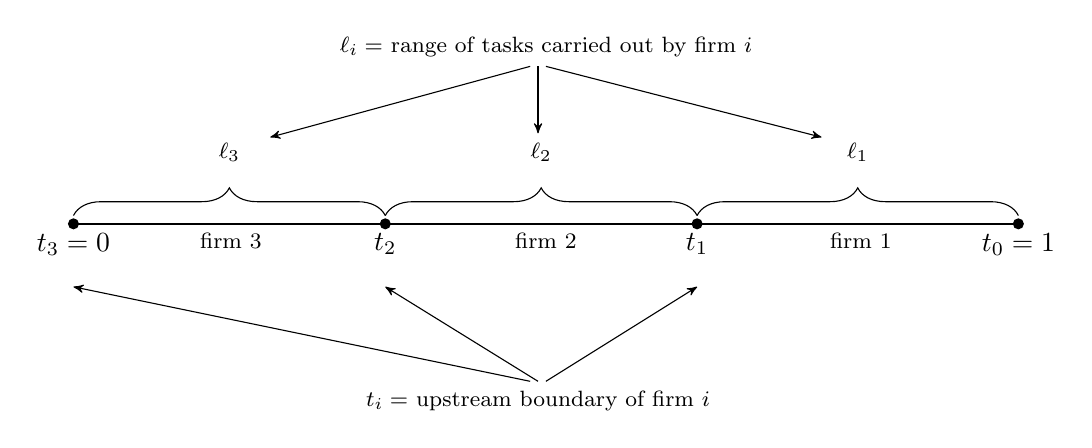
\begin{tikzpicture}[scale=1]

  \def\linelen{12}
  \def\tone{0.66 * \linelen};
  \def\ttwo{0.33 * \linelen};

  \draw[thick] (0,0) -- (\linelen,0);

  \fill (0,0) circle (2pt) node [below] {$t_3 = 0$};
  \fill (\linelen,0) circle (2pt) node [below] {$t_0 = 1$};
  \fill (\tone,0) circle (2pt) node [below] {$t_1$};
  \fill (\ttwo,0) circle (2pt) node [below] {$t_2$};

  \draw [decorate,decoration={brace,amplitude=10pt},xshift=0pt,yshift=3pt]
(0,0) -- (\ttwo,0) node [black,midway,yshift=0.8cm] {\footnotesize
$\ell_3$};

  \draw [decorate,decoration={brace,amplitude=10pt},xshift=0pt,yshift=3pt]
(\ttwo,0) -- (\tone,0) node [black,midway,yshift=0.8cm] {\footnotesize
$\ell_2$};

  \draw [decorate,decoration={brace,amplitude=10pt},xshift=0pt,yshift=3pt]
(\tone,0) -- (\linelen,0) node [black,midway,yshift=0.8cm] {\footnotesize
$\ell_1$};

\node at (10, 0) [below] {\footnotesize firm 1};
\node at (6, 0) [below] {\footnotesize firm 2};
\node at (2, 0) [below] {\footnotesize firm 3};

% Notation on in-house production and firm boundaries
\def\a{2};
\draw[->] (5.9, \a) -- (5.9, 1.15) ;
\draw[->] (6, \a) node [above] {\footnotesize $\ell_i = $ range of tasks
carried out by firm $i$} -- (9.5, 1.1) ;
\draw[->] (5.8, \a) -- (2.5, 1.1) ;

\def\b{-2};
\draw[->] (6, \b) -- (\tone, -0.8) ;
\draw[->] (5.9, \b) node [below] {\footnotesize $t_i = $ upstream boundary
of firm $i$} -- (\ttwo, -0.8) ;
\draw[->] (5.8, \b) -- (0, -0.8) ;

\end{tikzpicture}


\end{document}
